\documentclass[]{article}
\usepackage{lmodern}
\usepackage{amssymb,amsmath}
\usepackage{ifxetex,ifluatex}
\usepackage{fixltx2e} % provides \textsubscript
\ifnum 0\ifxetex 1\fi\ifluatex 1\fi=0 % if pdftex
  \usepackage[T1]{fontenc}
  \usepackage[utf8]{inputenc}
\else % if luatex or xelatex
  \ifxetex
    \usepackage{mathspec}
  \else
    \usepackage{fontspec}
  \fi
  \defaultfontfeatures{Ligatures=TeX,Scale=MatchLowercase}
\fi
% use upquote if available, for straight quotes in verbatim environments
\IfFileExists{upquote.sty}{\usepackage{upquote}}{}
% use microtype if available
\IfFileExists{microtype.sty}{%
\usepackage{microtype}
\UseMicrotypeSet[protrusion]{basicmath} % disable protrusion for tt fonts
}{}
\usepackage[margin=1in]{geometry}
\usepackage{hyperref}
\hypersetup{unicode=true,
            pdftitle={Laborator 3},
            pdfborder={0 0 0},
            breaklinks=true}
\urlstyle{same}  % don't use monospace font for urls
\usepackage{color}
\usepackage{fancyvrb}
\newcommand{\VerbBar}{|}
\newcommand{\VERB}{\Verb[commandchars=\\\{\}]}
\DefineVerbatimEnvironment{Highlighting}{Verbatim}{commandchars=\\\{\}}
% Add ',fontsize=\small' for more characters per line
\usepackage{framed}
\definecolor{shadecolor}{RGB}{248,248,248}
\newenvironment{Shaded}{\begin{snugshade}}{\end{snugshade}}
\newcommand{\AlertTok}[1]{\textcolor[rgb]{0.94,0.16,0.16}{#1}}
\newcommand{\AnnotationTok}[1]{\textcolor[rgb]{0.56,0.35,0.01}{\textbf{\textit{#1}}}}
\newcommand{\AttributeTok}[1]{\textcolor[rgb]{0.77,0.63,0.00}{#1}}
\newcommand{\BaseNTok}[1]{\textcolor[rgb]{0.00,0.00,0.81}{#1}}
\newcommand{\BuiltInTok}[1]{#1}
\newcommand{\CharTok}[1]{\textcolor[rgb]{0.31,0.60,0.02}{#1}}
\newcommand{\CommentTok}[1]{\textcolor[rgb]{0.56,0.35,0.01}{\textit{#1}}}
\newcommand{\CommentVarTok}[1]{\textcolor[rgb]{0.56,0.35,0.01}{\textbf{\textit{#1}}}}
\newcommand{\ConstantTok}[1]{\textcolor[rgb]{0.00,0.00,0.00}{#1}}
\newcommand{\ControlFlowTok}[1]{\textcolor[rgb]{0.13,0.29,0.53}{\textbf{#1}}}
\newcommand{\DataTypeTok}[1]{\textcolor[rgb]{0.13,0.29,0.53}{#1}}
\newcommand{\DecValTok}[1]{\textcolor[rgb]{0.00,0.00,0.81}{#1}}
\newcommand{\DocumentationTok}[1]{\textcolor[rgb]{0.56,0.35,0.01}{\textbf{\textit{#1}}}}
\newcommand{\ErrorTok}[1]{\textcolor[rgb]{0.64,0.00,0.00}{\textbf{#1}}}
\newcommand{\ExtensionTok}[1]{#1}
\newcommand{\FloatTok}[1]{\textcolor[rgb]{0.00,0.00,0.81}{#1}}
\newcommand{\FunctionTok}[1]{\textcolor[rgb]{0.00,0.00,0.00}{#1}}
\newcommand{\ImportTok}[1]{#1}
\newcommand{\InformationTok}[1]{\textcolor[rgb]{0.56,0.35,0.01}{\textbf{\textit{#1}}}}
\newcommand{\KeywordTok}[1]{\textcolor[rgb]{0.13,0.29,0.53}{\textbf{#1}}}
\newcommand{\NormalTok}[1]{#1}
\newcommand{\OperatorTok}[1]{\textcolor[rgb]{0.81,0.36,0.00}{\textbf{#1}}}
\newcommand{\OtherTok}[1]{\textcolor[rgb]{0.56,0.35,0.01}{#1}}
\newcommand{\PreprocessorTok}[1]{\textcolor[rgb]{0.56,0.35,0.01}{\textit{#1}}}
\newcommand{\RegionMarkerTok}[1]{#1}
\newcommand{\SpecialCharTok}[1]{\textcolor[rgb]{0.00,0.00,0.00}{#1}}
\newcommand{\SpecialStringTok}[1]{\textcolor[rgb]{0.31,0.60,0.02}{#1}}
\newcommand{\StringTok}[1]{\textcolor[rgb]{0.31,0.60,0.02}{#1}}
\newcommand{\VariableTok}[1]{\textcolor[rgb]{0.00,0.00,0.00}{#1}}
\newcommand{\VerbatimStringTok}[1]{\textcolor[rgb]{0.31,0.60,0.02}{#1}}
\newcommand{\WarningTok}[1]{\textcolor[rgb]{0.56,0.35,0.01}{\textbf{\textit{#1}}}}
\usepackage{longtable,booktabs}
\usepackage{graphicx,grffile}
\makeatletter
\def\maxwidth{\ifdim\Gin@nat@width>\linewidth\linewidth\else\Gin@nat@width\fi}
\def\maxheight{\ifdim\Gin@nat@height>\textheight\textheight\else\Gin@nat@height\fi}
\makeatother
% Scale images if necessary, so that they will not overflow the page
% margins by default, and it is still possible to overwrite the defaults
% using explicit options in \includegraphics[width, height, ...]{}
\setkeys{Gin}{width=\maxwidth,height=\maxheight,keepaspectratio}
\IfFileExists{parskip.sty}{%
\usepackage{parskip}
}{% else
\setlength{\parindent}{0pt}
\setlength{\parskip}{6pt plus 2pt minus 1pt}
}
\setlength{\emergencystretch}{3em}  % prevent overfull lines
\providecommand{\tightlist}{%
  \setlength{\itemsep}{0pt}\setlength{\parskip}{0pt}}
\setcounter{secnumdepth}{5}
% Redefines (sub)paragraphs to behave more like sections
\ifx\paragraph\undefined\else
\let\oldparagraph\paragraph
\renewcommand{\paragraph}[1]{\oldparagraph{#1}\mbox{}}
\fi
\ifx\subparagraph\undefined\else
\let\oldsubparagraph\subparagraph
\renewcommand{\subparagraph}[1]{\oldsubparagraph{#1}\mbox{}}
\fi

%%% Use protect on footnotes to avoid problems with footnotes in titles
\let\rmarkdownfootnote\footnote%
\def\footnote{\protect\rmarkdownfootnote}

%%% Change title format to be more compact
\usepackage{titling}

% Create subtitle command for use in maketitle
\providecommand{\subtitle}[1]{
  \posttitle{
    \begin{center}\large#1\end{center}
    }
}

\setlength{\droptitle}{-2em}

  \title{Laborator 3}
    \pretitle{\vspace{\droptitle}\centering\huge}
  \posttitle{\par}
  \subtitle{Elemente de probabilități și simulare în R}
  \author{}
    \preauthor{}\postauthor{}
    \date{}
    \predate{}\postdate{}
  
\usepackage{booktabs}
\usepackage{longtable}
\usepackage{framed,color}
\definecolor{shadecolor}{RGB}{248, 248, 248}
\definecolor{shadecolor1}{RGB}{216,225,235}
\definecolor{framecolor}{RGB}{16,111,124}%108,123,13

%\definecolor{shadecolor}{RGB}{226, 255, 241}
% \definecolor{shadecolor1}{RGB}{217,225,199}
% \definecolor{framecolor}{RGB}{60,179,113}

%%%%%%%%%%%%%%%%%%%%%%
\ifxetex
  \usepackage{letltxmacro}
  \setlength{\XeTeXLinkMargin}{1pt}
  \LetLtxMacro\SavedIncludeGraphics\includegraphics
  \def\includegraphics#1#{% #1 catches optional stuff (star/opt. arg.)
    \IncludeGraphicsAux{#1}%
  }%
  \newcommand*{\IncludeGraphicsAux}[2]{%
    \XeTeXLinkBox{%
      \SavedIncludeGraphics#1{#2}%
    }%
  }%
\fi

\newenvironment{frshaded*}{%
  \def\FrameCommand{\fboxrule=\FrameRule\fboxsep=\FrameSep \fcolorbox{framecolor}{shadecolor1}}%
  \MakeFramed {\advance\hsize-\width \FrameRestore}}%
{\endMakeFramed}

\newenvironment{rmdblock}[1]
  {\begin{frshaded*}
  \begin{itemize}
  \renewcommand{\labelitemi}{
    \raisebox{-.7\height}[0pt][0pt]{
      {\setkeys{Gin}{width=2em,keepaspectratio}\includegraphics{images/icons/#1}}
    }
  }
  \item
  }
  {
  \end{itemize}
  \end{frshaded*}
  }
  
%%%%%%%%%%%%%%%
% definitions.
% -------------------
\usepackage{marginnote}
% \renewcommand*{\marginnotevadjust}{40pt}
% \renewcommand{\marginnotevadjust}{0pt}
% \renewcommand{\marginfont}{\noindent\rule{0pt}{0.7\baselineskip}\tiny}

\newtheorem{proposition}{Proposition}[section]
\newtheorem{lemma}[proposition]{Lemma}
\newtheorem{corollary}[proposition]{Corollary}
\newtheorem{theorem}[proposition]{Theorem}

\newcounter{exo}[section]
\newcommand{\enonce}[2]{\refstepcounter{proposition}\hypertarget{exo:#1}{}\label{exo:#1}{\scriptsize\;\textbf{Ex.}~\ref{exo:#1}}}

\reversemarginpar
\setlength{\marginparwidth}{1.2cm}
% 
% \newcommand{\enonce}[2]{\refstepcounter{proposition}\hypertarget{exo:#1}{}\label{exo:#1}{\noindent\color{black}\normalsize\bf Exercice \ref{exo:#1}}\ \  #2\vspace{1mm}\hrule\vspace{1mm} \color{black}\normalsize}


%%%%%%%%%%%%%%%

% \newenvironment{rmdcaution}
%   {\begin{rmdblock}{caution}}
%   {\end{rmdblock}}

% \newenvironment{rmdinsight}
%   {\begin{rmdblock}{insight}}
%   {\end{rmdblock}}

\newenvironment{rmdexercise}
  {\begin{rmdblock}{exercise}}
  {\end{rmdblock}}

% \newenvironment{rmdexercise_tex}
%   {\begin{rmdblock}{exercise}}
%   {\end{rmdblock}}
  
% \newenvironment{rmdtip}
%   {\begin{rmdblock}{tip}}
%   {\end{rmdblock}}


%%%%%%%%%%%%%%%%%%%%%%%%%%%%%%%%%%%%%%%%%%%%%%%%%%%%%%%%%%%%%%%%%%%%%%%%%%%%%%%%%%%%%%%%%%%%%%%%%%%%%%%%%%%%%%%%%%%%%
%%%%%%%%%%% For insight block %%%%%%%%%%%%%%%%%%%%%%%%%%
\definecolor{shadecolor_insight}{RGB}{223,240,216}
\definecolor{framecolor_insight}{RGB}{136,193,137}

%\definecolor{shadecolor_insight}{RGB}{217,225,199}
%\definecolor{framecolor_insight}{RGB}{60,179,113}

\newenvironment{frshaded_insight*}{%
  \def\FrameCommand{\fboxrule=\FrameRule\fboxsep=\FrameSep \fcolorbox{framecolor_insight}{shadecolor_insight}}%
  \MakeFramed {\advance\hsize-\width \FrameRestore}}%
{\endMakeFramed}

\newenvironment{rmdblock_insight}[1]
  {\begin{frshaded_insight*}
  \begin{itemize}
  \renewcommand{\labelitemi}{
    \raisebox{-.7\height}[0pt][0pt]{
      {\setkeys{Gin}{width=2em,keepaspectratio}\includegraphics{images/icons/#1}}
    }
  }
  \item
  }
  {
  \end{itemize}
  \end{frshaded_insight*}
  }

\newenvironment{rmdinsight}
  {\begin{rmdblock_insight}{insight}}
  {\end{rmdblock_insight}}

%%%%%%%%%%% For caution block %%%%%%%%%%%%%%%%%%%%%%%%%%
\definecolor{shadecolor_caution}{RGB}{250,250,250}
\definecolor{framecolor_caution}{RGB}{242,129,67}%193,75,34

\newenvironment{frshaded_caution*}{%
  \def\FrameCommand{\fboxrule=\FrameRule\fboxsep=\FrameSep \fcolorbox{framecolor_caution}{shadecolor_caution}}%
  \MakeFramed {\advance\hsize-\width \FrameRestore}}%
{\endMakeFramed}

\newenvironment{rmdblock_caution}[1]
  {\begin{frshaded_caution*}
  \begin{itemize}
  \renewcommand{\labelitemi}{
    \raisebox{-.7\height}[0pt][0pt]{
      {\setkeys{Gin}{width=2em,keepaspectratio}\includegraphics{images/icons/#1}}
    }
  }
  \item
  }
  {
  \end{itemize}
  \end{frshaded_caution*}
  }
  
\newenvironment{rmdcaution}
  {\begin{rmdblock_caution}{caution}}
  {\end{rmdblock_caution}}

%%%%%%%%%%% For tip block %%%%%%%%%%%%%%%%%%%%%%%%%%
\definecolor{shadecolor_tip}{RGB}{250,250,250}
\definecolor{framecolor_tip}{RGB}{33,153,195}

\newenvironment{frshaded_tip*}{%
  \def\FrameCommand{\fboxrule=\FrameRule\fboxsep=\FrameSep \fcolorbox{framecolor_tip}{shadecolor_tip}}%
  \MakeFramed {\advance\hsize-\width \FrameRestore}}%
{\endMakeFramed}

\newenvironment{rmdblock_tip}[1]
  {\begin{frshaded_tip*}
  \begin{itemize}
  \renewcommand{\labelitemi}{
    \raisebox{-.7\height}[0pt][0pt]{
      {\setkeys{Gin}{width=2em,keepaspectratio}\includegraphics{images/icons/#1}}
    }
  }
  \item
  }
  {
  \end{itemize}
  \end{frshaded_tip*}
  }
  
\newenvironment{rmdtip}
  {\begin{rmdblock_tip}{tip}}
  {\end{rmdblock_tip}}

%%%%%%%%%%%%%%%%%%%%%%%%%%%%%%%%%%%%%%%%%%%%%%%%%%%%%%%%%%%%%%%%%%%%%%%%%%%%%%%%%%%%%%%%%%%%%%%%%%%%%%%%%%%%%%%%%%%%%
\usepackage{subfigure}
\usepackage{booktabs}
\usepackage{slashbox}
\usepackage{color}
%%%%%%%%%%%%%%%%%%%%%%%%%%%%%%%%%%%%%%%%%
\definecolor{linkcol}{rgb}{0,0,0.4}
\definecolor{citecol}{rgb}{0.5,0,0}

% Change this to change the informations included in the pdf file
% \usepackage[pagebackref]{hyperref}
% \usepackage[verbose]{backref}
\usepackage[hyperpageref]{backref}
% \backrefsetup{verbose=false}
% \PassOptionsToPackage{pagebackref}{hyperref}
% See hyperref documentation for information on those parameters

\hypersetup
{
bookmarksopen=true,
pdftitle="Curs Statistica",
pdfauthor="Alexandru Amarioarei",
pdfsubject="Curs Statistica", %subject of the document
pdfmenubar=true, %menubar shown
pdfhighlight=/O, %effect of clicking on a link
colorlinks=true, %couleurs sur les liens hypertextes
pdfpagemode=None, %aucun mode de page
pdfpagelayout=SinglePage, %ouverture en simple page
pdffitwindow=true, %pages ouvertes entierement dans toute la fenetre
linkcolor=linkcol, %couleur des liens hypertextes internes
citecolor=citecol, %couleur des liens pour les citations
urlcolor=linkcol %couleur des liens pour les url
}


% set the back references
\renewcommand*{\backref}[1]{}
\renewcommand*{\backreftwosep}{ și~} % inserted between entries 
                              % in a list of two entries, 
                              % default is " and~".
\renewcommand*{\backreflastsep}{ și~} % inserted between the last 
                               % two entries of a list with more
                               % than two entries, default is ", and~".
\renewcommand*{\backrefalt}[4]{%
    \ifcase #1 (Necitat.)%
    \or        (Citat la pagina~#2.)%
    \else      (Citat la paginile~#2.)%
    \fi}

%%%%%%%%%%%%%%%%%%%%%%%%%%%%%%%%%%%%%%%%%%%%%%%%%%%%%%%%%%%%%%%%%%%%%%%%%%%%%%%%%%%%%%%%%%%%%%%%%%%%%%%%%%%%%%%%%%%%%
%CITEVA DEFINITII
\def\om{\omega}
\def\Om{\Omega}
\def\et{\eta}
\def\td{\tilde{\delta}}
\def\m{{\mu}}
\def\n{{\nu}}
\def\k{{\kappa}}
\def\l{{\lambda}}
\def\L{{\Lambda}}
\def\g{{\gamma}}
\def\a{{\alpha}}
\def\e{{\varepsilon}}
\def\b{{\beta}}
\def\G{{\Gamma}}
\def\d{{\delta}}
\def\D{{\Delta}}
\def\t{{\theta}}
\def\s{{\sigma}}
\def\S{{\Sigma}}
\def\z{{\zeta}}
\def\qed{\hfill\Box}
\def\ds{\displaystyle}
\def\mc{\mathcal}
%%%%%%%%%%%%%%%%%%%%%%%%%%%%%%%%%%%%%%%%%%%%%%%%%%%%%%%%%%%%%%%%%%%%%%%%%%%%%%%%%%%%%%%%%%%%%%%%%%%%%%%%%%%%%%%%%%%%%%
\def\1{{\mathbf 1}}
\def\CC{{\mathbb C}}
\def\VV{{\mathbb V}}
\def\RR{{\mathbb R}}
\def\QQ{{\mathbb Q}}
\def\ZZ{{\mathbb Z}}
\def\PP{{\mathbb P}}
\def\EE{{\mathbb E}}
\def\NN{{\mathbb N}}
\def\FF{{\mathbb F}}
%\def\SS{{\mathbb S}}
\def\MA{{\mathcal A}}
\def\MO{{\mathcal O}}
\def\MF{{\mathcal F}}
\def\ME{{\mathcal E}}
\def\MR{{\mathcal R}}
\def\MB{{\mathcal B}}
\def\MM{{\mathcal M}}
\def\MN{{\mathcal N}}
\def\MU{{\mathcal U}}
\def\MP{{\mathcal P}}
\def\MS{{\mathcal S}}
\def\MBS{{\mathbf S}}
\def\MX{{\bm{ \mathscr X}}}

% independent sign
\newcommand\independent{\protect\mathpalette{\protect\independenT}{\perp}}
\def\independenT#1#2{\mathrel{\rlap{$#1#2$}\mkern2mu{#1#2}}}

\renewcommand\tablename{Tab.}
\renewcommand{\figurename}{Fig.}
\renewcommand\refname{Referințe}

%%%%%%%%%%%%%%%%%%%%%%%%%%%%%%%%%%%%%%%%%%%%%%%%%%%%%%%%%%%%%%%%%%%%%%%%%%%%%%%%%%%%%%%%%%%%%%%%%%%%%%%%%%%%%%%%%%%%%
%Header and Footer
\usepackage{fancyhdr}

\pagestyle{fancy}
\fancyhf{}
\rhead{Universitatea din Bucure\c sti\\ Facultatea de Matematic\u a \c si Informatic\u a}
% \lhead{\textit{Curs}: Tehnici alternative în predarea matematicii (2018)\\ \textit{Instructori}: A. Am\u arioarei, M. Patriche}
\lhead{\textit{Curs}: Statistică (2019-2020)\\ \textit{Instructori}: A. Am\u arioarei, S. Cojocea}
\rfoot{Pagina \thepage}
\lfoot{Grupele: 301, 311, 321}
%%%%%%%%%%%%%%%%%%%%%%%%%%%%%%%%%%%%%%%
%%%%%%%%%%%%%%%%%%%%%%%%%%%%%%%%%%%%%%%
\usepackage{pifont}% http://ctan.org/pkg/pifont
\newcommand{\cmark}{\ding{51}}%
\newcommand{\xmark}{\ding{55}}%
\usepackage{booktabs}
\usepackage{longtable}
\usepackage{array}
\usepackage{multirow}
\usepackage{wrapfig}
\usepackage{float}
\usepackage{colortbl}
\usepackage{pdflscape}
\usepackage{tabu}
\usepackage{threeparttable}
\usepackage{threeparttablex}
\usepackage[normalem]{ulem}
\usepackage{makecell}
\usepackage{xcolor}

\begin{document}
\maketitle

%%%%%%%%%%%%%%%%%%%%%%%%
\thispagestyle{fancy}

Obiectivul acestui laborator este de a prezenta succint câteva funcții
utile teoriei probabilităților din programul
\href{https://cran.r-project.org/}{R}, care este structura lor și cum le
putem aplica. De asemenea, tot în acest laborator vom prezenta și câteva
probleme de simulare punând accent pe rezultatele de bază din teoria
probabilităților și anume \emph{Legea Numerelor Mari} și \emph{Teorema
Limită Centrală}.

\hypertarget{familia-de-funcux21bii-apply}{%
\section{\texorpdfstring{Familia de funcții
\texttt{apply}}{Familia de funcții apply}}\label{familia-de-funcux21bii-apply}}

Pe lângă buclele \texttt{for} și \texttt{while}, în R există și un set
de funcții care permit scrierea și rularea într-o manieră mai compactă a
codului dar și aplicarea de funcții unor grupuri de date.

\begin{itemize}
\item
  \texttt{lapply()}: Evaluează o funcție pentru fiecare element al unei
  liste
\item
  \texttt{sapply()}: La fel ca \texttt{lapply} numai că încearcă să
  simplifice rezultatul
\item
  \texttt{apply()}: Aplică o funcție după fiecare dimensiune a unui
  \texttt{array}
\item
  \texttt{tapply()}: Aplică o funcție pe submulțimi ale unui vector
\item
  \texttt{mapply()}: Varianta multivariată a funcției \texttt{lapply}
\item
  \texttt{split}: Împarte un vector în grupuri definite de o variabilă
  de tip factor.
\end{itemize}

\hypertarget{lapply}{%
\subsection{\texorpdfstring{\texttt{lapply()}}{lapply()}}\label{lapply}}

Funcția \texttt{lapply()} efectuează următoarele operații:

\begin{enumerate}
\def\labelenumi{\arabic{enumi}.}
\tightlist
\item
  buclează după o listă, iterând după fiecare element din acea listă
\item
  aplică o \emph{funcție} fiecărui element al listei (o funcție pe care
  o specificăm)
\item
  întoarce ca rezultat tot o listă (prefixul \texttt{l} vine de la
  listă).
\end{enumerate}

Această funcție primește următoarele trei argument: (1) o listă
\texttt{X}; (2) o funcție \texttt{FUN}; (3) alte argumente via
\texttt{...}. Dacă \texttt{X} nu este o listă atunci aceasta va fi
transformată într-una folosind comanda \texttt{as.list()}.

Considerăm următorul exemplu în care vrem să aplicăm funcția
\texttt{mean()} tuturor elementelor unei liste

\begin{Shaded}
\begin{Highlighting}[]
\KeywordTok{set.seed}\NormalTok{(}\DecValTok{222}\NormalTok{)}
\NormalTok{x <-}\StringTok{ }\KeywordTok{list}\NormalTok{(}\DataTypeTok{a =} \DecValTok{1}\OperatorTok{:}\DecValTok{5}\NormalTok{, }\DataTypeTok{b =} \KeywordTok{rnorm}\NormalTok{(}\DecValTok{10}\NormalTok{), }\DataTypeTok{c =} \KeywordTok{rnorm}\NormalTok{(}\DecValTok{20}\NormalTok{, }\DecValTok{1}\NormalTok{), }\DataTypeTok{d =} \KeywordTok{rnorm}\NormalTok{(}\DecValTok{100}\NormalTok{, }\DecValTok{5}\NormalTok{))}
\KeywordTok{lapply}\NormalTok{(x, mean)}
\OperatorTok{$}\NormalTok{a}
\NormalTok{[}\DecValTok{1}\NormalTok{] }\DecValTok{3}

\OperatorTok{$}\NormalTok{b}
\NormalTok{[}\DecValTok{1}\NormalTok{] }\FloatTok{0.1996044}

\OperatorTok{$}\NormalTok{c}
\NormalTok{[}\DecValTok{1}\NormalTok{] }\FloatTok{0.7881026}

\OperatorTok{$}\NormalTok{d}
\NormalTok{[}\DecValTok{1}\NormalTok{] }\FloatTok{5.064188}
\end{Highlighting}
\end{Shaded}

Putem să folosim funcția \texttt{lapply()} pentru a evalua o funcție în
moduri repetate. Mai jos avem un exemplu în care folosim funcția
\texttt{runif()} (permite generarea observațiilor uniform repartizate)
de patru ori, de fiecare dată generăm un număr diferit de valori
aleatoare. Mai mult, argumentele \(min=0\) și \(max=3\) sunt atribuite,
prin intermediul argumentului \texttt{...}, funcției \texttt{runif}.

\begin{Shaded}
\begin{Highlighting}[]
\NormalTok{x <-}\StringTok{ }\DecValTok{1}\OperatorTok{:}\DecValTok{4}
\KeywordTok{lapply}\NormalTok{(x, runif, }\DataTypeTok{min =} \DecValTok{0}\NormalTok{, }\DataTypeTok{max =} \DecValTok{3}\NormalTok{)}
\NormalTok{[[}\DecValTok{1}\NormalTok{]]}
\NormalTok{[}\DecValTok{1}\NormalTok{] }\FloatTok{0.03443616}

\NormalTok{[[}\DecValTok{2}\NormalTok{]]}
\NormalTok{[}\DecValTok{1}\NormalTok{] }\FloatTok{1.267361} \FloatTok{1.365441}

\NormalTok{[[}\DecValTok{3}\NormalTok{]]}
\NormalTok{[}\DecValTok{1}\NormalTok{] }\FloatTok{1.8084700} \FloatTok{2.1902665} \FloatTok{0.4139585}

\NormalTok{[[}\DecValTok{4}\NormalTok{]]}
\NormalTok{[}\DecValTok{1}\NormalTok{] }\FloatTok{1.5924650} \FloatTok{0.7355067} \FloatTok{2.1483841} \FloatTok{1.6082945}
\end{Highlighting}
\end{Shaded}

\hypertarget{sapply}{%
\subsection{\texorpdfstring{\texttt{sapply()}}{sapply()}}\label{sapply}}

Funcția \texttt{sapply()} are un comportament similar cu
\texttt{lapply()} prin faptul că funcția \texttt{sapply()} apelează
intern \texttt{lapply()} pentru valorile de input, după care evaluează:

\begin{itemize}
\item
  dacă rezultatul este o listă în care fiecare element este de lungime
  1, atunci întoarce un vector
\item
  dacă rezultatul este o listă în care fiecare element este un vector de
  aceeași lungime (\textgreater1), se întoarce o matrice
\item
  în caz contrar se întoarce o listă.
\end{itemize}

Considerăm exemplul de mai sus

\begin{Shaded}
\begin{Highlighting}[]
\KeywordTok{set.seed}\NormalTok{(}\DecValTok{222}\NormalTok{)}
\NormalTok{x <-}\StringTok{ }\KeywordTok{list}\NormalTok{(}\DataTypeTok{a =} \DecValTok{1}\OperatorTok{:}\DecValTok{4}\NormalTok{, }\DataTypeTok{b =} \KeywordTok{rnorm}\NormalTok{(}\DecValTok{10}\NormalTok{), }\DataTypeTok{c =} \KeywordTok{rnorm}\NormalTok{(}\DecValTok{20}\NormalTok{, }\DecValTok{1}\NormalTok{), }\DataTypeTok{d =} \KeywordTok{rnorm}\NormalTok{(}\DecValTok{100}\NormalTok{, }\DecValTok{5}\NormalTok{))}
\KeywordTok{sapply}\NormalTok{(x, mean)}
\NormalTok{        a         b         c         d }
\FloatTok{2.5000000} \FloatTok{0.1996044} \FloatTok{0.7881026} \FloatTok{5.0641876} 
\end{Highlighting}
\end{Shaded}

\hypertarget{split}{%
\subsection{\texorpdfstring{\texttt{split()}}{split()}}\label{split}}

Funcția \texttt{split()} primește ca argument un vector sau o listă (sau
un data.frame) și împarte datele în grupuri determinate de o variabilă
de tip factor (sau o listă de factor).

Argumentele aceste funcții sunt

\begin{Shaded}
\begin{Highlighting}[]
\KeywordTok{str}\NormalTok{(split)}
\ControlFlowTok{function}\NormalTok{ (x, f, }\DataTypeTok{drop =} \OtherTok{FALSE}\NormalTok{, ...)  }
\end{Highlighting}
\end{Shaded}

unde

\begin{itemize}
\tightlist
\item
  \texttt{x} este un vector, o listă sau un data.frame
\item
  \texttt{f} este un factor sau o listă de factori
\end{itemize}

Considerăm următorul exemplu în care generăm un vector de date și îl
împărțim după o variabilă de tip factor creată cu ajutorul funcției
\texttt{gl()} (\emph{generate levels}).

\begin{Shaded}
\begin{Highlighting}[]
\NormalTok{x <-}\StringTok{ }\KeywordTok{c}\NormalTok{(}\KeywordTok{rnorm}\NormalTok{(}\DecValTok{10}\NormalTok{), }\KeywordTok{runif}\NormalTok{(}\DecValTok{10}\NormalTok{), }\KeywordTok{rnorm}\NormalTok{(}\DecValTok{10}\NormalTok{, }\DecValTok{1}\NormalTok{))}
\NormalTok{f <-}\StringTok{ }\KeywordTok{gl}\NormalTok{(}\DecValTok{3}\NormalTok{, }\DecValTok{10}\NormalTok{)}
\KeywordTok{split}\NormalTok{(x, f)}
\OperatorTok{$}\StringTok{`}\DataTypeTok{1}\StringTok{`}
\NormalTok{ [}\DecValTok{1}\NormalTok{] }\FloatTok{-2.27414224} \FloatTok{-0.11266780}  \FloatTok{0.61308167}  \FloatTok{0.07733545}  \FloatTok{0.57137727}
\NormalTok{ [}\DecValTok{6}\NormalTok{]  }\FloatTok{0.11672493} \FloatTok{-0.95685256} \FloatTok{-1.90008460} \FloatTok{-1.48972089}  \FloatTok{0.55925676}

\OperatorTok{$}\StringTok{`}\DataTypeTok{2}\StringTok{`}
\NormalTok{ [}\DecValTok{1}\NormalTok{] }\FloatTok{0.91159086} \FloatTok{0.03291829} \FloatTok{0.78368939} \FloatTok{0.11852882} \FloatTok{0.64443831} \FloatTok{0.78790988}
\NormalTok{ [}\DecValTok{7}\NormalTok{] }\FloatTok{0.82451477} \FloatTok{0.05642366} \FloatTok{0.65075027} \FloatTok{0.95426854}

\OperatorTok{$}\StringTok{`}\DataTypeTok{3}\StringTok{`}
\NormalTok{ [}\DecValTok{1}\NormalTok{]  }\FloatTok{2.6666242}  \FloatTok{2.6634334}  \FloatTok{1.8106280} \FloatTok{-0.7837308}  \FloatTok{1.6575684}  \FloatTok{0.1546575}
\NormalTok{ [}\DecValTok{7}\NormalTok{]  }\FloatTok{0.4930056} \FloatTok{-0.9031544}  \FloatTok{2.4042311}  \FloatTok{1.4106863}
\end{Highlighting}
\end{Shaded}

Putem folosi funcția \texttt{split} și în conjuncție cu funcția
\texttt{lapply} (atunci când vrem să aplicăm o funcție \texttt{FUN} pe
grupuri de date).

\begin{Shaded}
\begin{Highlighting}[]
\KeywordTok{lapply}\NormalTok{(}\KeywordTok{split}\NormalTok{(x, f), mean)}
\OperatorTok{$}\StringTok{`}\DataTypeTok{1}\StringTok{`}
\NormalTok{[}\DecValTok{1}\NormalTok{] }\FloatTok{-0.4795692}

\OperatorTok{$}\StringTok{`}\DataTypeTok{2}\StringTok{`}
\NormalTok{[}\DecValTok{1}\NormalTok{] }\FloatTok{0.5765033}

\OperatorTok{$}\StringTok{`}\DataTypeTok{3}\StringTok{`}
\NormalTok{[}\DecValTok{1}\NormalTok{] }\FloatTok{1.157395}
\end{Highlighting}
\end{Shaded}

\hypertarget{tapply}{%
\subsection{\texorpdfstring{\texttt{tapply()}}{tapply()}}\label{tapply}}

Funcția \texttt{tapply()} este folosită pentru aplicarea unei funcții
\texttt{FUN} pe submulțimile unui vector și poate fi văzută ca o
combinație între \texttt{split()} și \texttt{sapply()}, dar doar pentru
vectori.

\begin{Shaded}
\begin{Highlighting}[]
\KeywordTok{str}\NormalTok{(tapply)}
\ControlFlowTok{function}\NormalTok{ (X, INDEX, }\DataTypeTok{FUN =} \OtherTok{NULL}\NormalTok{, ..., }\DataTypeTok{default =} \OtherTok{NA}\NormalTok{, }\DataTypeTok{simplify =} \OtherTok{TRUE}\NormalTok{)  }
\end{Highlighting}
\end{Shaded}

Argumentele acestei funcții sunt date de următorul tabel:

\begin{longtable}[]{@{}ll@{}}
\caption{Argumentele functiei tapply}\tabularnewline
\toprule
Argument & Descriere\tabularnewline
\midrule
\endfirsthead
\toprule
Argument & Descriere\tabularnewline
\midrule
\endhead
\texttt{X} & un vector\tabularnewline
\texttt{INDEX} & este o variabilă de tip factor sau o listă de
factori\tabularnewline
\texttt{FUN} & o funcție ce urmează să fie aplicată\tabularnewline
\texttt{...} & argumente ce vor fi atribuite funcției
\texttt{FUN}\tabularnewline
\texttt{simplify} & dacă vrem să simplificăm rezultatul\tabularnewline
\bottomrule
\end{longtable}

Următorul exemplu calculează media după fiecare grupă determinată de o
variabilă de tip factor a unui vector numeric.

\begin{Shaded}
\begin{Highlighting}[]
\NormalTok{x <-}\StringTok{ }\KeywordTok{c}\NormalTok{(}\KeywordTok{rnorm}\NormalTok{(}\DecValTok{10}\NormalTok{), }\KeywordTok{runif}\NormalTok{(}\DecValTok{10}\NormalTok{), }\KeywordTok{rnorm}\NormalTok{(}\DecValTok{10}\NormalTok{, }\DecValTok{1}\NormalTok{))}
\NormalTok{f <-}\StringTok{ }\KeywordTok{gl}\NormalTok{(}\DecValTok{3}\NormalTok{, }\DecValTok{10}\NormalTok{)   }
\NormalTok{f}
\NormalTok{ [}\DecValTok{1}\NormalTok{] }\DecValTok{1} \DecValTok{1} \DecValTok{1} \DecValTok{1} \DecValTok{1} \DecValTok{1} \DecValTok{1} \DecValTok{1} \DecValTok{1} \DecValTok{1} \DecValTok{2} \DecValTok{2} \DecValTok{2} \DecValTok{2} \DecValTok{2} \DecValTok{2} \DecValTok{2} \DecValTok{2} \DecValTok{2} \DecValTok{2} \DecValTok{3} \DecValTok{3} \DecValTok{3} \DecValTok{3} \DecValTok{3} \DecValTok{3} \DecValTok{3} \DecValTok{3} \DecValTok{3} \DecValTok{3}
\NormalTok{Levels}\OperatorTok{:}\StringTok{ }\DecValTok{1} \DecValTok{2} \DecValTok{3}
\KeywordTok{tapply}\NormalTok{(x, f, mean)}
            \DecValTok{1}             \DecValTok{2}             \DecValTok{3} 
\FloatTok{-0.0007774025}  \FloatTok{0.3736457792}  \FloatTok{0.5789436983} 
\end{Highlighting}
\end{Shaded}

Putem să aplicăm și funcții care întorc mai mult de un rezultat. În
această situație rezultatul nu poate fi simplificat:

\begin{Shaded}
\begin{Highlighting}[]
\KeywordTok{tapply}\NormalTok{(x, f, range)}
\OperatorTok{$}\StringTok{`}\DataTypeTok{1}\StringTok{`}
\NormalTok{[}\DecValTok{1}\NormalTok{] }\FloatTok{-2.1904113}  \FloatTok{0.9249901}

\OperatorTok{$}\StringTok{`}\DataTypeTok{2}\StringTok{`}
\NormalTok{[}\DecValTok{1}\NormalTok{] }\FloatTok{0.004445296} \FloatTok{0.998309704}

\OperatorTok{$}\StringTok{`}\DataTypeTok{3}\StringTok{`}
\NormalTok{[}\DecValTok{1}\NormalTok{] }\FloatTok{-0.3379675}  \FloatTok{1.9327099}
\end{Highlighting}
\end{Shaded}

\hypertarget{apply}{%
\subsection{\texorpdfstring{\texttt{apply()}}{apply()}}\label{apply}}

Funcția \texttt{apply()} este folosită cu precădere pentru a aplica o
funcție liniilor și coloanelor unei matrice (care este un \texttt{array}
bidimensional). Cu toate acestea poate fi folosită pe tablouri
multidimensionale (\texttt{array}) în general. Folosirea funcției
\texttt{apply()} nu este mai rapidă decât scrierea unei bucle
\texttt{for}, dar este mai compactă.

\begin{Shaded}
\begin{Highlighting}[]
\KeywordTok{str}\NormalTok{(apply)}
\ControlFlowTok{function}\NormalTok{ (X, MARGIN, FUN, ...)  }
\end{Highlighting}
\end{Shaded}

Argumentele funcției \texttt{apply()} sunt

\begin{itemize}
\tightlist
\item
  \texttt{X} un tablou multidimensional
\item
  \texttt{MARGIN} este un vector numeric care indică dimensiunea sau
  dimensiunile după care se va aplica funcția
\item
  \texttt{FUN} este o funcție ce urmează să fie aplicată
\item
  \texttt{...} alte argumente penru funcția\texttt{FUN}
\end{itemize}

Considerăm următorul exemplu în care calculăm media pe coloane într-o
matrice

\begin{Shaded}
\begin{Highlighting}[]
\NormalTok{x <-}\StringTok{ }\KeywordTok{matrix}\NormalTok{(}\KeywordTok{rnorm}\NormalTok{(}\DecValTok{200}\NormalTok{), }\DecValTok{20}\NormalTok{, }\DecValTok{10}\NormalTok{)}
\KeywordTok{apply}\NormalTok{(x, }\DecValTok{2}\NormalTok{, mean)  }\CommentTok{## media fiecarei coloane}
\NormalTok{ [}\DecValTok{1}\NormalTok{]  }\FloatTok{3.745002e-02}  \FloatTok{1.857656e-01} \FloatTok{-2.413659e-01} \FloatTok{-2.093141e-01} \FloatTok{-2.562272e-01}
\NormalTok{ [}\DecValTok{6}\NormalTok{]  }\FloatTok{8.986712e-05}  \FloatTok{7.444137e-02} \FloatTok{-7.460941e-03}  \FloatTok{6.275282e-02}  \FloatTok{9.801550e-02}
\end{Highlighting}
\end{Shaded}

precum și media după fiecare linie

\begin{Shaded}
\begin{Highlighting}[]
\KeywordTok{apply}\NormalTok{(x, }\DecValTok{1}\NormalTok{, sum)   }\CommentTok{## media fiecarei linii}
\NormalTok{ [}\DecValTok{1}\NormalTok{]  }\FloatTok{2.76179139}  \FloatTok{2.53107681}  \FloatTok{0.87923177}  \FloatTok{1.80480589}  \FloatTok{0.98225832}
\NormalTok{ [}\DecValTok{6}\NormalTok{] }\FloatTok{-3.06148753} \FloatTok{-1.40358820} \FloatTok{-0.65969812} \FloatTok{-1.63717046} \FloatTok{-0.29330726}
\NormalTok{[}\DecValTok{11}\NormalTok{] }\FloatTok{-2.41486442} \FloatTok{-3.15698523}  \FloatTok{2.27126822} \FloatTok{-3.88290287} \FloatTok{-3.15595194}
\NormalTok{[}\DecValTok{16}\NormalTok{]  }\FloatTok{5.41211963}  \FloatTok{2.32985530} \FloatTok{-3.05330574} \FloatTok{-0.02110926} \FloatTok{-1.34909559}
\end{Highlighting}
\end{Shaded}

\hypertarget{repartiux21bii-ux219i-elemente-aleatoare-uxeen-r}{%
\section{Repartiții și elemente aleatoare în
R}\label{repartiux21bii-ux219i-elemente-aleatoare-uxeen-r}}

R pune la disploziție majoritatea repartițiilor uzuale. Tabelul de mai
jos prezintă numele și parametrii acestora:

\begin{longtable}[]{@{}llll@{}}
\caption{Numele si parametrii repartitiilor uzuale in R}\tabularnewline
\toprule
Repartiția & Nume & Parametrii & Valori prestabilite\tabularnewline
\midrule
\endfirsthead
\toprule
Repartiția & Nume & Parametrii & Valori prestabilite\tabularnewline
\midrule
\endhead
Beta & \texttt{beta} & \texttt{shape1}, \texttt{shape2} &\tabularnewline
Binomial & \texttt{binom} & \texttt{size}, \texttt{prob}
&\tabularnewline
Cauchy & \texttt{cauchy} & \texttt{location}, \texttt{scale} &
\texttt{location\ =\ 0}, \texttt{scale\ =\ 1}\tabularnewline
Chi-Squared & \texttt{chisq} & \texttt{df} &\tabularnewline
Exponential & \texttt{exp} & \texttt{rate} (=1/mean) &
\texttt{rate\ =\ 1}\tabularnewline
Fisher & \texttt{f} & \texttt{df1}, \texttt{df2} &\tabularnewline
Gamma & \texttt{gamma} & \texttt{shape}, \texttt{rate} (=1/scale) &
\texttt{rate\ =\ 1}\tabularnewline
Hypergeometric & \texttt{hyper} & \texttt{m}, \texttt{n}, \texttt{k}
&\tabularnewline
Log-Normal & \texttt{lnorm} & \texttt{mean}, \texttt{sd} &
\texttt{mean\ =\ 0}, \texttt{sd\ =\ 1}\tabularnewline
Logistic & \texttt{logis} & \texttt{location}, \texttt{scale} &
\texttt{location\ =\ 0}, \texttt{scale\ =\ 1}\tabularnewline
Normal & \texttt{norm} & \texttt{mean}, \texttt{sd} &
\texttt{mean\ =\ 0}, \texttt{sd\ =\ 1}\tabularnewline
Poisson & \texttt{pois} & \texttt{lambda} &\tabularnewline
Student & \texttt{t} & \texttt{df} &\tabularnewline
Uniform & \texttt{unif} & \texttt{min}, \texttt{max} &
\texttt{min\ =\ 0}, \texttt{max\ =\ 1}\tabularnewline
Weibull & \texttt{weibull} & \texttt{shape} &\tabularnewline
\bottomrule
\end{longtable}

Pentru fiecare repartiție, există patru comenzi în R prefixate cu
literele \texttt{d}, \texttt{p}, \texttt{q} și \texttt{r} și urmate de
numele repartiției (coloana a 2-a). De exemplu \texttt{dnorm},
\texttt{pnorm}, \texttt{qnorm} și \texttt{rnorm} sunt comenzile
corespunzătoare repartiției normale pe când \texttt{dunif},
\texttt{punif}, \texttt{qunif} și \texttt{runif} sunt cele
corespunzătoare repartiției uniforme.

\begin{itemize}
\item
  \texttt{dname}: calculează densitatea atunci când vorbim de o
  variabilă continue sau funcția de masă atunci când avem o repartiție
  discretă (\(\mathbb{P}(X=k)\))
\item
  \texttt{pname}: calculează funcția de repartiție,
  i.e.~\(F(x)=\mathbb{P}(X\leq x)\)
\item
  \texttt{qname}: reprezintă funcția cuantilă, cu alte cuvinte valoarea
  pentru care funcția de repartiție are o anumită probabilitate; în
  cazul continuu, dacă \texttt{pname(x)\ =\ p} atunci
  \texttt{qname(p)\ =\ x} iar în cazul discret întoarce cel mai mic
  întreg \(u\) pentru care \(\mathbb{P}(X\leq u)\geq p\).
\item
  \texttt{rname}: generează observații independente din repartiția dată
\end{itemize}

Avem următoarele exemple:

\begin{Shaded}
\begin{Highlighting}[]
\KeywordTok{qnorm}\NormalTok{(}\FloatTok{0.975}\NormalTok{)}
\NormalTok{[}\DecValTok{1}\NormalTok{] }\FloatTok{1.959964}
\KeywordTok{pnorm}\NormalTok{(}\FloatTok{1.96}\NormalTok{)}
\NormalTok{[}\DecValTok{1}\NormalTok{] }\FloatTok{0.9750021}
\KeywordTok{rnorm}\NormalTok{(}\DecValTok{5}\NormalTok{)}
\NormalTok{[}\DecValTok{1}\NormalTok{] }\FloatTok{0.4304737} \FloatTok{0.8405027} \FloatTok{1.9550682} \FloatTok{1.6208507} \FloatTok{2.1059503}

\NormalTok{x =}\StringTok{ }\KeywordTok{seq}\NormalTok{(}\OperatorTok{-}\DecValTok{1}\NormalTok{, }\DecValTok{1}\NormalTok{, }\FloatTok{0.25}\NormalTok{)}
\KeywordTok{dnorm}\NormalTok{(x)}
\NormalTok{[}\DecValTok{1}\NormalTok{] }\FloatTok{0.2419707} \FloatTok{0.3011374} \FloatTok{0.3520653} \FloatTok{0.3866681} \FloatTok{0.3989423} \FloatTok{0.3866681} \FloatTok{0.3520653}
\NormalTok{[}\DecValTok{8}\NormalTok{] }\FloatTok{0.3011374} \FloatTok{0.2419707}
\KeywordTok{rnorm}\NormalTok{(}\DecValTok{3}\NormalTok{, }\DecValTok{5}\NormalTok{, }\FloatTok{0.5}\NormalTok{)}
\NormalTok{[}\DecValTok{1}\NormalTok{] }\FloatTok{5.327249} \FloatTok{4.728878} \FloatTok{5.773167}

\KeywordTok{dunif}\NormalTok{(x)}
\NormalTok{[}\DecValTok{1}\NormalTok{] }\DecValTok{0} \DecValTok{0} \DecValTok{0} \DecValTok{0} \DecValTok{1} \DecValTok{1} \DecValTok{1} \DecValTok{1} \DecValTok{1}
\KeywordTok{runif}\NormalTok{(}\DecValTok{3}\NormalTok{)}
\NormalTok{[}\DecValTok{1}\NormalTok{] }\FloatTok{0.6353840} \FloatTok{0.8470974} \FloatTok{0.0672359}
\end{Highlighting}
\end{Shaded}

\hypertarget{exerciux21bii-propuse}{%
\section{Exerciții propuse}\label{exerciux21bii-propuse}}

\hypertarget{aruncarea-cu-banul}{%
\subsection{Aruncarea cu banul}\label{aruncarea-cu-banul}}

În acest exemplu vrem să simulăm aruncarea unei monede (echilibrate)
folosind funcția \texttt{sample()}. Această funcție permite extragerea,
cu sau fără întoarcere (\texttt{replace\ =\ TRUE} sau
\texttt{replace\ =\ FALSE} - aceasta este valoarea prestabilită), a unui
eșantion de volum dat (\texttt{size}) dintr-o mulțime de elemente
\texttt{x}.

Spre exemplu dacă vrem să simulăm \(10\) aruncări cu banul atunci
apelăm:

\begin{Shaded}
\begin{Highlighting}[]
\KeywordTok{sample}\NormalTok{(}\KeywordTok{c}\NormalTok{(}\StringTok{"H"}\NormalTok{, }\StringTok{"T"}\NormalTok{), }\DecValTok{10}\NormalTok{, }\DataTypeTok{replace =} \OtherTok{TRUE}\NormalTok{)}
\NormalTok{ [}\DecValTok{1}\NormalTok{] }\StringTok{"T"} \StringTok{"T"} \StringTok{"T"} \StringTok{"T"} \StringTok{"T"} \StringTok{"T"} \StringTok{"T"} \StringTok{"H"} \StringTok{"H"} \StringTok{"T"}
\end{Highlighting}
\end{Shaded}

Pentru a estima probabilitatea de apariției a stemei (\texttt{H})
repetăm aruncarea cu banul de \(10000\) de ori și calculăm raportul
dintre numărul de apariții ale evenimentului \(A=\{H\}\) și numărul
total de aruncări:

\begin{Shaded}
\begin{Highlighting}[]
\CommentTok{# atunci cand moneda este echilibrata}
\NormalTok{a =}\StringTok{ }\KeywordTok{sample}\NormalTok{(}\KeywordTok{c}\NormalTok{(}\StringTok{"H"}\NormalTok{,}\StringTok{"T"}\NormalTok{), }\DecValTok{10000}\NormalTok{, }\DataTypeTok{replace =} \OtherTok{TRUE}\NormalTok{)}
\NormalTok{p =}\StringTok{ }\KeywordTok{sum}\NormalTok{(a }\OperatorTok{==}\StringTok{ "H"}\NormalTok{)}\OperatorTok{/}\KeywordTok{length}\NormalTok{(a)}
\NormalTok{p}
\NormalTok{[}\DecValTok{1}\NormalTok{] }\FloatTok{0.5073}
\end{Highlighting}
\end{Shaded}

și pentru cazul în care moneda nu este echilibrată

\begin{Shaded}
\begin{Highlighting}[]
\NormalTok{a =}\StringTok{ }\KeywordTok{sample}\NormalTok{(}\KeywordTok{c}\NormalTok{(}\StringTok{"H"}\NormalTok{,}\StringTok{"T"}\NormalTok{), }\DecValTok{10000}\NormalTok{, }\DataTypeTok{replace =} \OtherTok{TRUE}\NormalTok{, }\DataTypeTok{prob =} \KeywordTok{c}\NormalTok{(}\FloatTok{0.2}\NormalTok{, }\FloatTok{0.8}\NormalTok{))}
\NormalTok{p =}\StringTok{ }\KeywordTok{sum}\NormalTok{(a }\OperatorTok{==}\StringTok{ "H"}\NormalTok{)}\OperatorTok{/}\KeywordTok{length}\NormalTok{(a)}
\NormalTok{p}
\NormalTok{[}\DecValTok{1}\NormalTok{] }\FloatTok{0.2012}
\end{Highlighting}
\end{Shaded}

Putem vedea cum evoluează această probabilitatea în funcție de numărul
de repetări

\begin{Shaded}
\begin{Highlighting}[]
\NormalTok{y =}\StringTok{ }\KeywordTok{rep}\NormalTok{(}\DecValTok{0}\NormalTok{,}\DecValTok{100}\NormalTok{)}

\ControlFlowTok{for}\NormalTok{ (i }\ControlFlowTok{in} \DecValTok{1}\OperatorTok{:}\DecValTok{100}\NormalTok{)\{}
\NormalTok{  a =}\StringTok{ }\KeywordTok{sample}\NormalTok{(}\KeywordTok{c}\NormalTok{(}\StringTok{"H"}\NormalTok{,}\StringTok{"T"}\NormalTok{), i}\OperatorTok{*}\DecValTok{100}\NormalTok{, }\DataTypeTok{replace =} \OtherTok{TRUE}\NormalTok{)}
\NormalTok{  y[i] =}\StringTok{ }\KeywordTok{sum}\NormalTok{(a }\OperatorTok{==}\StringTok{ "H"}\NormalTok{)}\OperatorTok{/}\KeywordTok{length}\NormalTok{(a)}
\NormalTok{\}}

\KeywordTok{plot}\NormalTok{(}\DecValTok{1}\OperatorTok{:}\DecValTok{100}\NormalTok{, y, }\DataTypeTok{type =} \StringTok{"o"}\NormalTok{, }\DataTypeTok{col =}\NormalTok{ myblue, }\DataTypeTok{bty =} \StringTok{"n"}\NormalTok{,}
     \DataTypeTok{xlab =}\StringTok{""}\NormalTok{, }\DataTypeTok{ylab =} \StringTok{"probabilitatea"}\NormalTok{)}
\KeywordTok{abline}\NormalTok{(}\DataTypeTok{h =} \FloatTok{0.5}\NormalTok{, }\DataTypeTok{lty =} \DecValTok{2}\NormalTok{, }\DataTypeTok{col =}\NormalTok{ myred)}
\end{Highlighting}
\end{Shaded}

\begin{center}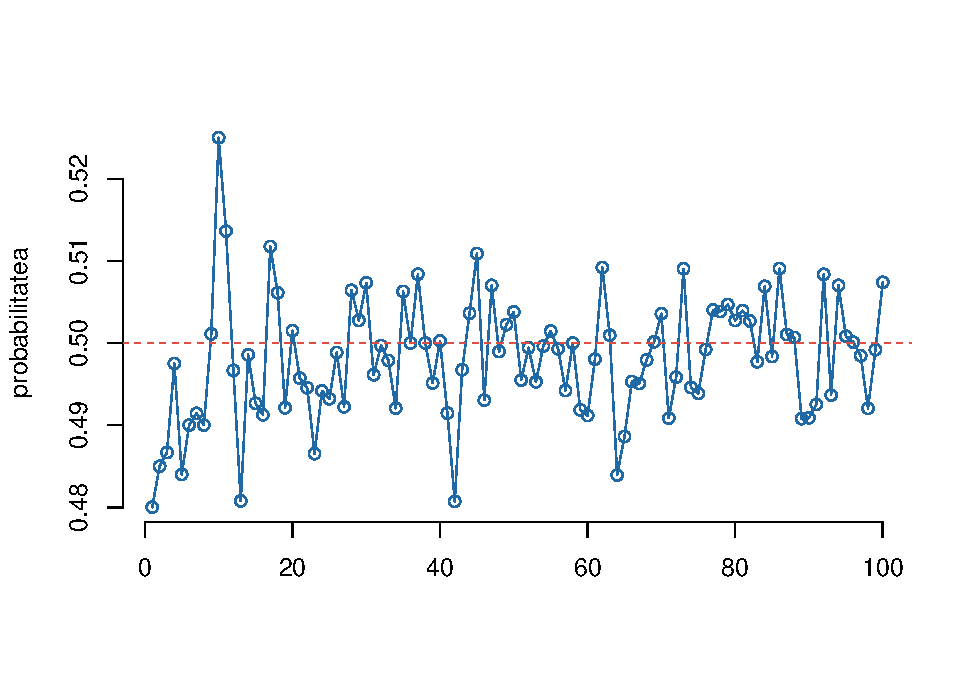
\includegraphics[width=0.8\linewidth]{Lab3_files/figure-latex/unnamed-chunk-19-1} \end{center}

\hypertarget{jocul-de-loto}{%
\subsection{Jocul de loto}\label{jocul-de-loto}}

\begin{rmdexercise}
Construiți în R o funcție care să simuleze jocul de loto \(6/49\). Acest
joc consistă din extragerea aleatoare a \(6\) numere dintr-o urnă cu
\(49\) de numere posibile, fără întoarcere. Fiecare extragere se face de
manieră uniformă din numerele rămase în urnă (la a i-a extragere fiecare
bilă din urnă are aceeași șansă să fie extrasă). De exemplu putem avea
următorul rezultat: \(10, 27, 3, 45, 12, 24\).

\textbf{Notă}: Funcția \texttt{sample()} poate face această operație,
ceea ce se cere este de a crea voi o funcție care să implementeze jocul
fără a folosi funcția \emph{sample}. Binențeles că puteți folosi funcții
precum: \texttt{runif} , \texttt{floor}, \texttt{choose}, etc.
\end{rmdexercise}

Începem prin a construi o funcție care ne permite generarea unei
variabile aleatoare uniform repartizate pe mulțimea \(\{1,2,\dots,n\}\)
(această funcție este cea care simulează procesul de extragere de la
fiecare pas):

\begin{Shaded}
\begin{Highlighting}[]
\NormalTok{myintunif =}\StringTok{ }\ControlFlowTok{function}\NormalTok{(n)\{}
  \CommentTok{# dunctia care genereaza un numar uniform intre 1 si n}
\NormalTok{  r =}\StringTok{ }\NormalTok{n}\OperatorTok{*}\KeywordTok{runif}\NormalTok{(}\DecValTok{1}\NormalTok{)}
\NormalTok{  u =}\StringTok{ }\KeywordTok{floor}\NormalTok{(r)}\OperatorTok{+}\DecValTok{1}
  \KeywordTok{return}\NormalTok{(u)}
\NormalTok{\}}
\end{Highlighting}
\end{Shaded}

Funcția care realizează extragerea fără întoarcere a \(k\) numere
aleatoare din \(n\), este:

\begin{Shaded}
\begin{Highlighting}[]
\NormalTok{myrandsample=}\ControlFlowTok{function}\NormalTok{(n,k)\{}
  \CommentTok{# }
\NormalTok{  x =}\StringTok{ }\DecValTok{1}\OperatorTok{:}\NormalTok{n}
\NormalTok{  q =}\StringTok{ }\KeywordTok{rep}\NormalTok{(}\DecValTok{0}\NormalTok{,k)}
  
  \ControlFlowTok{for}\NormalTok{(i }\ControlFlowTok{in} \DecValTok{1}\OperatorTok{:}\NormalTok{k)\{}
\NormalTok{    l =}\StringTok{ }\KeywordTok{length}\NormalTok{(x)}
\NormalTok{    u =}\StringTok{ }\KeywordTok{myintunif}\NormalTok{(l)}
\NormalTok{    q[i] =}\StringTok{ }\NormalTok{x[u]}
\NormalTok{    x =}\StringTok{ }\NormalTok{x[x}\OperatorTok{!=}\NormalTok{q[i]]}
\NormalTok{  \}}
  \KeywordTok{return}\NormalTok{(q)}
\NormalTok{\}}
\end{Highlighting}
\end{Shaded}

Pentru a vedea ce face această funcție putem scrie:

\begin{Shaded}
\begin{Highlighting}[]
\NormalTok{n =}\StringTok{ }\DecValTok{49}
\NormalTok{k =}\StringTok{ }\DecValTok{6}

\KeywordTok{myrandsample}\NormalTok{(n,k)}
\NormalTok{[}\DecValTok{1}\NormalTok{]  }\DecValTok{3} \DecValTok{16} \DecValTok{12} \DecValTok{48} \DecValTok{23} \DecValTok{32}
\end{Highlighting}
\end{Shaded}

\hypertarget{ilustrarea-legii-numerelor-mari}{%
\subsection{Ilustrarea Legii Numerelor
Mari}\label{ilustrarea-legii-numerelor-mari}}

\begin{rmdexercise}
\begin{enumerate}
\def\labelenumi{\alph{enumi})}
\item
  Fie \(X_1,X_2,\dots,X_N\), \(N\) v.a. i.i.d. de lege
  \(\mathcal{U}([0,1])\). Pentru \(1\leq n\leq N\), notăm cu
  \(S_n=X_1+X_2+\cdots X_n\) șirul sumelor parțiale și \(\mu\) media
  legii \(\mathcal{U}([0,1])\). Trasați pe același grafic funcția
  \(n\to \frac{S_n}{n}\) pentru \(n=1,\dots,N\) și dreapta de ecuație
  \(y=\mu\). Faceți același lucru pentru legea normală
  \(\mathcal{N}(2,1)\).
\item
  Utilizați \emph{Legea Numerelor Mari} pentru a aproxima integrala
  următoarez
\end{enumerate}

\[I = \int_{0}^{1}e^{x}sin(2x)cos(2x)dx.\]

Calculați de asemenea valoarea exactă \(I\) a acesteia și comparați-o cu
aproximarea găsită.
\end{rmdexercise}

\begin{enumerate}
\def\labelenumi{\alph{enumi})}
\tightlist
\item
  În cazul în care v.a. \(X_1,X_2,\dots,X_N\) sunt repartizate uniform
  \(\mathcal{U}([0,1])\) (deci media este \(\mu=\frac{1}{2}\)) avem:
\end{enumerate}

\begin{Shaded}
\begin{Highlighting}[]
\NormalTok{n =}\StringTok{ }\DecValTok{10000}

\CommentTok{# Pentru legea uniforma folosim comanda runif}
\CommentTok{# Pentru calculul sumelor partiale putem folosi functia cumsum}

\NormalTok{y1 =}\StringTok{ }\KeywordTok{cumsum}\NormalTok{(}\KeywordTok{runif}\NormalTok{(n))}
\NormalTok{y1 =}\StringTok{ }\NormalTok{y1}\OperatorTok{/}\NormalTok{(}\DecValTok{1}\OperatorTok{:}\NormalTok{n)}
\NormalTok{mu1 =}\StringTok{ }\DecValTok{1}\OperatorTok{/}\DecValTok{2} \CommentTok{# media uniformei pe [0,1]}

\CommentTok{# trasam graficul }
\KeywordTok{plot}\NormalTok{(}\DecValTok{1}\OperatorTok{:}\NormalTok{n, y1, }\DataTypeTok{type =} \StringTok{"l"}\NormalTok{, }
     \DataTypeTok{col=}\NormalTok{ myblue, }\DataTypeTok{xlab =} \StringTok{"n"}\NormalTok{, }
     \DataTypeTok{ylab =} \KeywordTok{expression}\NormalTok{(S[n]), }
     \DataTypeTok{bty =} \StringTok{"n"}\NormalTok{)}
\KeywordTok{abline}\NormalTok{(}\DataTypeTok{h =}\NormalTok{ mu1, }\DataTypeTok{col =}\NormalTok{ myred, }\DataTypeTok{lty=} \StringTok{"dashed"}\NormalTok{) }\CommentTok{# adaugam linia orizontala}
\end{Highlighting}
\end{Shaded}

\begin{figure}

{\centering 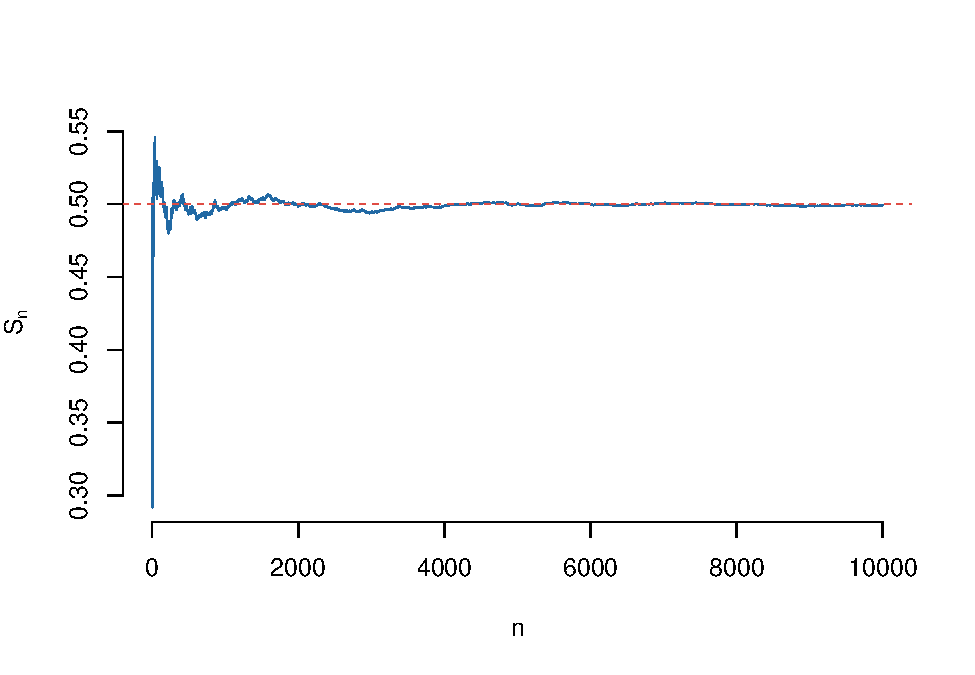
\includegraphics[width=0.8\linewidth]{Lab3_files/figure-latex/unnamed-chunk-25-1} 

}

\caption{Ilustrarea legii numerelor mari: v.a. uniforme}\label{fig:unnamed-chunk-25}
\end{figure}

În cazul în care v.a. \(X_1,X_2,\dots,X_N\) sunt normale de parametrii
\(\mathcal{N}(2,1)\) (deci media este \(\mu=2\)) avem:

\begin{Shaded}
\begin{Highlighting}[]
\CommentTok{# Folosim acelasi numar de variabile n}

\CommentTok{# Pentru legea normala folosim comanda rnorm}
\CommentTok{# Pentru calculul sumelor partiale putem folosi functia cumsum}
\NormalTok{y2 =}\StringTok{ }\KeywordTok{cumsum}\NormalTok{(}\KeywordTok{rnorm}\NormalTok{(n, }\DataTypeTok{mean =} \DecValTok{2}\NormalTok{, }\DataTypeTok{sd =} \DecValTok{1}\NormalTok{))}
\NormalTok{y2 =}\StringTok{ }\NormalTok{y2}\OperatorTok{/}\NormalTok{(}\DecValTok{1}\OperatorTok{:}\NormalTok{n)}
\NormalTok{mu2 =}\StringTok{ }\DecValTok{2} \CommentTok{# media normalei N(2,1)}

\CommentTok{# facem graficul }
\KeywordTok{plot}\NormalTok{(}\DecValTok{1}\OperatorTok{:}\NormalTok{n, y2, }\DataTypeTok{type =} \StringTok{"l"}\NormalTok{, }
     \DataTypeTok{col=}\NormalTok{ myblue, }\DataTypeTok{xlab =} \StringTok{"n"}\NormalTok{, }
     \DataTypeTok{ylab =} \KeywordTok{expression}\NormalTok{(S[n]),}
     \DataTypeTok{bty =} \StringTok{"n"}\NormalTok{)}
\KeywordTok{abline}\NormalTok{(}\DataTypeTok{h =}\NormalTok{ mu2, }\DataTypeTok{col =}\NormalTok{ myred, }\DataTypeTok{lty=} \StringTok{"dashed"}\NormalTok{) }\CommentTok{# adaugam linia orizontala}
\end{Highlighting}
\end{Shaded}

\begin{figure}

{\centering 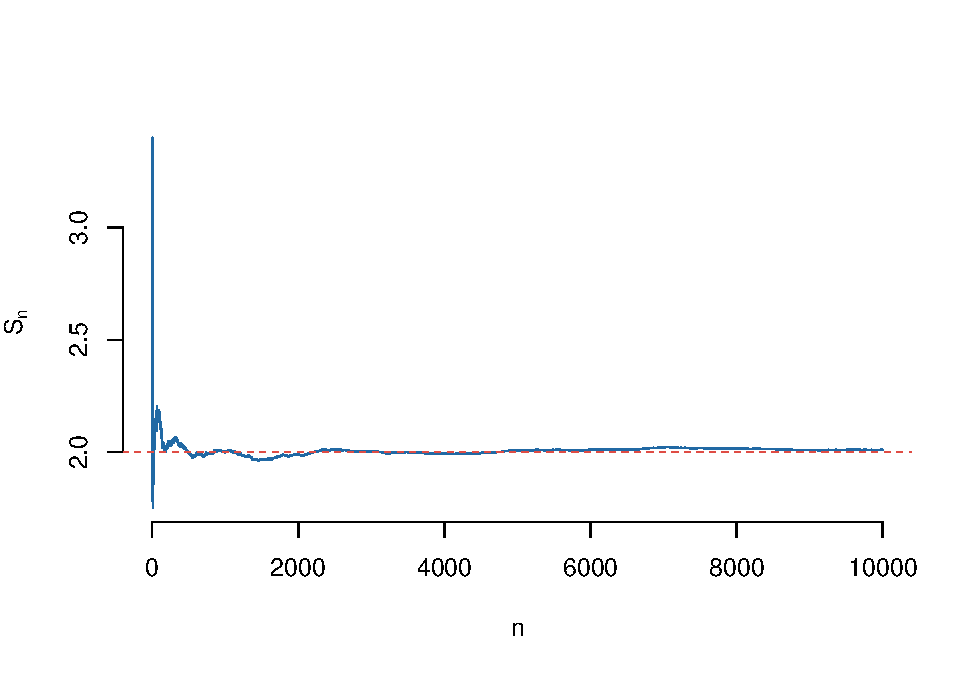
\includegraphics[width=0.8\linewidth]{Lab3_files/figure-latex/unnamed-chunk-26-1} 

}

\caption{Ilustrarea legii numerelor mari: v.a. normale}\label{fig:unnamed-chunk-26}
\end{figure}

\begin{enumerate}
\def\labelenumi{\alph{enumi})}
\setcounter{enumi}{1}
\tightlist
\item
  Fie \(U_1,U_2,\dots,U_n\) un șir de v.a. i.i.d. repartizare uniform pe
  \([0,1]\). Cum \(g\) este o funcție continuă, aplicând \emph{Legea
  Numerelor Mari} obținem
\end{enumerate}

\[
  g_n=\frac{1}{n}\sum_{i=1}^{n}g(U_{i}) \overset{a.s.}{\to} \mathbb{E}[g(U_1)] = \int_{0}^{1}g(x)dx.
\]

Pentru a calcula integrala numeric vom folosi funcția \texttt{integrate}
(trebuie observat că această integrală se poate calcula ușor și exact
prin integrare prin părți). Următorul script ne dă valoare numerică și
aproximarea obținută cu ajutorul metodei Monte Carlo pentru integrale
\(\int_{0}^{1}g(x)dx\):

\begin{Shaded}
\begin{Highlighting}[]
\NormalTok{myfun=}\ControlFlowTok{function}\NormalTok{(x)\{}
\NormalTok{  y =}\StringTok{ }\KeywordTok{exp}\NormalTok{(x)}\OperatorTok{*}\KeywordTok{sin}\NormalTok{(}\DecValTok{2}\OperatorTok{*}\NormalTok{x)}\OperatorTok{*}\KeywordTok{cos}\NormalTok{(}\DecValTok{2}\OperatorTok{*}\NormalTok{x);}
  \KeywordTok{return}\NormalTok{(y);}
\NormalTok{\}}

\CommentTok{# calculul integralei cu metode numerice}
\NormalTok{I =}\StringTok{ }\KeywordTok{integrate}\NormalTok{(myfun,}\DecValTok{0}\NormalTok{,}\DecValTok{1}\NormalTok{) }\CommentTok{# raspunsul este o lista si oprim prima valoare}
\NormalTok{I =}\StringTok{ }\NormalTok{I[}\DecValTok{1}\NormalTok{]}

\CommentTok{# calculul integralei cu ajutorul metodei Monte Carlo}
\NormalTok{n =}\StringTok{ }\DecValTok{10000} 

\NormalTok{u =}\StringTok{ }\KeywordTok{runif}\NormalTok{(n) }\CommentTok{# generarea sirului U_n}
\NormalTok{z =}\StringTok{ }\KeywordTok{myfun}\NormalTok{(u) }\CommentTok{# calcularea sirului g_n}

\NormalTok{I2 =}\StringTok{ }\KeywordTok{sum}\NormalTok{(z)}\OperatorTok{/}\NormalTok{n }\CommentTok{# aproximarea MC}
\end{Highlighting}
\end{Shaded}

Obținem că valoarea numerică a lui \(I\) este 0.2662 iar cea obținută cu
ajutorul metodei Monte Carlo este 0.2591.

Avem următoarea ilustrare grafică a convergenței metodei Monte Carlo:

\begin{Shaded}
\begin{Highlighting}[]
\CommentTok{# graficul}
\NormalTok{gn =}\StringTok{ }\KeywordTok{myfun}\NormalTok{(}\KeywordTok{runif}\NormalTok{(n)) }
\NormalTok{gn =}\StringTok{ }\KeywordTok{cumsum}\NormalTok{(gn)}\OperatorTok{/}\NormalTok{(}\DecValTok{1}\OperatorTok{:}\NormalTok{n) }\CommentTok{# calculul lui g_n}

\KeywordTok{plot}\NormalTok{(}\DecValTok{1}\OperatorTok{:}\NormalTok{n, gn, }\DataTypeTok{type =} \StringTok{"l"}\NormalTok{, }
     \DataTypeTok{col =}\NormalTok{ myblue, }\DataTypeTok{xlab =} \StringTok{"n"}\NormalTok{, }
     \DataTypeTok{ylab =} \KeywordTok{expression}\NormalTok{(g[n]),}
     \DataTypeTok{bty =} \StringTok{"n"}\NormalTok{)}
\KeywordTok{abline}\NormalTok{(}\DataTypeTok{h =}\NormalTok{ I, }\DataTypeTok{lty =} \StringTok{"dashed"}\NormalTok{, }\DataTypeTok{col =}\NormalTok{ myred)}
\end{Highlighting}
\end{Shaded}

\begin{figure}

{\centering 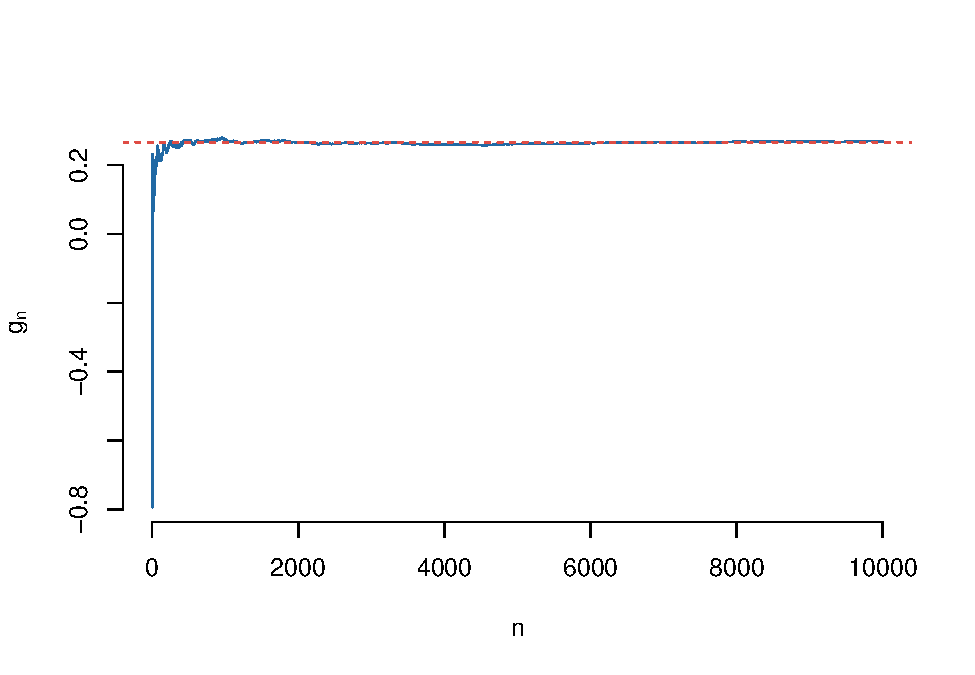
\includegraphics[width=0.8\linewidth]{Lab3_files/figure-latex/unnamed-chunk-28-1} 

}

\caption{Convergenta metodei Monte Carlo (pentru g)}\label{fig:unnamed-chunk-28}
\end{figure}

\hypertarget{ilustrarea-teoremei-limitux103-centralux103-i}{%
\subsection{Ilustrarea Teoremei Limită Centrală
(I)}\label{ilustrarea-teoremei-limitux103-centralux103-i}}

\begin{rmdexercise}
Fie \((X_n)_{n\geq1}\) un șir de v.a. i.i.d. de lege \(\mathcal{E}(1)\).
Pentru toți \(n\), notăm cu \(S_n=X_1+X_2+\cdots X_n\) șirul sumelor
parțiale, \(\mu\) și \(\sigma^2\) reprezentând media și respectiv
varianța legii \(\mathcal{E}(1)\). \emph{Teorema Limită Centrală} afirmă
că dacă \(n\) este mare atunci v.a.

\[
\frac{S_n-n\mu}{\sqrt{n}\sigma}
\]

are aproximativ aceeași distribuție ca și legea normală
\(\mathcal{N}(0,1)\). Ilustrați această convergență în distribuție cu
ajutorul unei histograme (i.e.~simulând un număr mare de realizări
independente ale v.a. \(\frac{S_n-n\mu}{\sqrt{n}\sigma}\)). Suprapuneți
peste această histogramă densitatea legii \(\mathcal{N}(0,1)\).
\end{rmdexercise}

Știm că media unei v.a. distribuite exponențial de parametru
\(\lambda\), \(\mathcal{E}(\lambda)\) este \(\mu=\frac{1}{\lambda}\) iar
varianța acesteia este \(\sigma^2=\frac{1}{\lambda^2}\). Pentru fiecare
valoare a lui \(i\) de la \(1\) la \(N\) calculăm raportul
\(\frac{S_n-n\mu}{\sigma\sqrt{n}}\) (cu alte cuvinte repetăm
experimentul de \(N\) ori):

\begin{Shaded}
\begin{Highlighting}[]
\NormalTok{N =}\StringTok{ }\DecValTok{1000} \CommentTok{# alegem numarul de repetitii ale experimentului}
\NormalTok{n =}\StringTok{ }\DecValTok{1000} \CommentTok{# alegem n pentru care folosim aproximarea normala}

\NormalTok{lambda =}\StringTok{ }\DecValTok{1} \CommentTok{# parametrul legii E(1)}

\NormalTok{mu =}\StringTok{ }\DecValTok{1}\OperatorTok{/}\NormalTok{lambda }\CommentTok{# media}
\NormalTok{sigma =}\StringTok{ }\DecValTok{1}\OperatorTok{/}\NormalTok{lambda }\CommentTok{# abaterea standard }

\NormalTok{s =}\StringTok{ }\KeywordTok{rep}\NormalTok{(}\DecValTok{0}\NormalTok{,N) }\CommentTok{# initializam sirul sumelor partiale}

\ControlFlowTok{for}\NormalTok{ (i }\ControlFlowTok{in} \DecValTok{1}\OperatorTok{:}\NormalTok{N)\{}
\NormalTok{  x =}\StringTok{ }\KeywordTok{rexp}\NormalTok{(n, }\DataTypeTok{rate =}\NormalTok{ lambda) }\CommentTok{# generam variabilele exponentiale}
\NormalTok{  s[i] =}\StringTok{ }\NormalTok{(}\KeywordTok{sum}\NormalTok{(x)}\OperatorTok{-}\NormalTok{n}\OperatorTok{*}\NormalTok{mu)}\OperatorTok{/}\NormalTok{(sigma}\OperatorTok{*}\KeywordTok{sqrt}\NormalTok{(n)) }\CommentTok{# calculam raportul }
  
\NormalTok{\}}
\end{Highlighting}
\end{Shaded}

Continuăm prin trasarea histogramei cerute și adăugăm la grafic
densitatea legii normale \(\mathcal{N}(0,1)\):

\begin{Shaded}
\begin{Highlighting}[]
\CommentTok{# trasam histograma}
\CommentTok{# pentru mai multe optiuni latex: ?plotmath }
\KeywordTok{hist}\NormalTok{(s, }\DataTypeTok{main =} \KeywordTok{expression}\NormalTok{(}\KeywordTok{paste}\NormalTok{(}\StringTok{"Histograma raportului "}\NormalTok{,}\KeywordTok{frac}\NormalTok{(S[n]}\OperatorTok{-}\NormalTok{n}\OperatorTok\NormalTok{mu,sigma}\OperatorTok\KeywordTok{sqrt}\NormalTok{(n)))),}
     \DataTypeTok{prob =} \OtherTok{TRUE}\NormalTok{, }
     \DataTypeTok{col =}\NormalTok{ myblue, }\CommentTok{# Culoarea de umplere}
     \DataTypeTok{border =} \StringTok{"white"}\NormalTok{,}
     \DataTypeTok{xlim =} \KeywordTok{c}\NormalTok{(}\OperatorTok{-}\DecValTok{4}\NormalTok{,}\DecValTok{4}\NormalTok{), }
     \DataTypeTok{cex.main=}\FloatTok{0.75}\NormalTok{, }
     \DataTypeTok{cex.lab =} \FloatTok{0.75}\NormalTok{, }
     \DataTypeTok{cex.axis =} \FloatTok{0.75}\NormalTok{, }
     \DataTypeTok{xlab =} \StringTok{""}\NormalTok{, }
     \DataTypeTok{ylab =} \StringTok{"Densitatea"}\NormalTok{)}

\CommentTok{# adaugam densitatea normalei N(0,1) }
\NormalTok{x1 =}\StringTok{ }\KeywordTok{seq}\NormalTok{(}\OperatorTok{-}\DecValTok{4}\NormalTok{,}\DecValTok{4}\NormalTok{,}\DataTypeTok{by=}\FloatTok{0.1}\NormalTok{)}
\NormalTok{y1 =}\StringTok{ }\KeywordTok{dnorm}\NormalTok{(x1, }\DataTypeTok{mean =} \DecValTok{0}\NormalTok{, }\DataTypeTok{sd =} \DecValTok{1}\NormalTok{)}
\KeywordTok{lines}\NormalTok{(x1, y1, }\DataTypeTok{col =}\NormalTok{ myred, }\DataTypeTok{lwd =} \DecValTok{2}\NormalTok{, }\DataTypeTok{lty =} \DecValTok{2}\NormalTok{)}
\end{Highlighting}
\end{Shaded}

\begin{figure}

{\centering 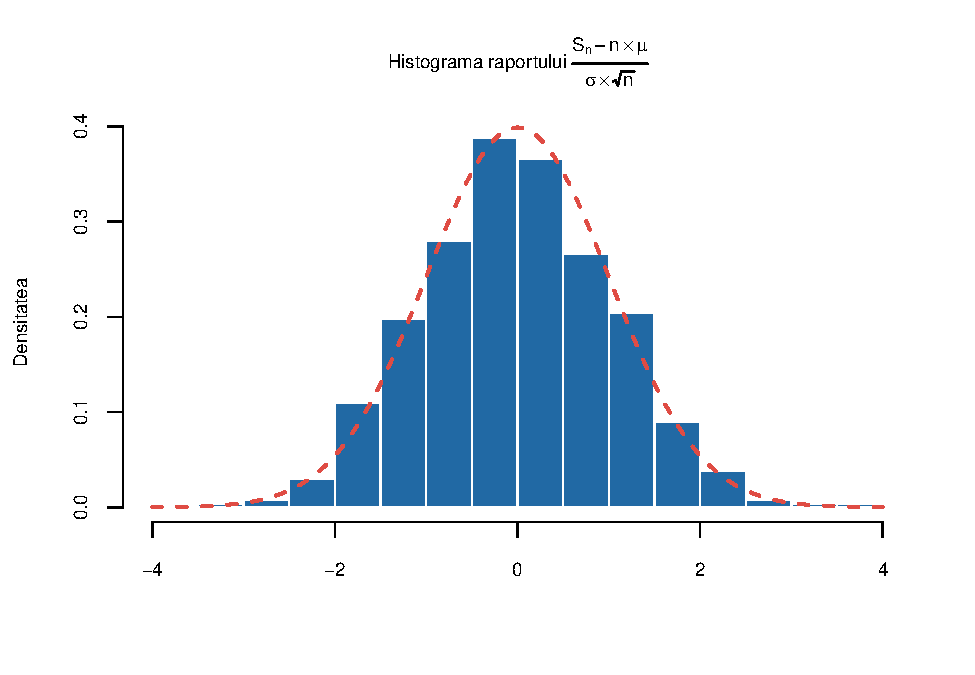
\includegraphics[width=0.8\linewidth]{Lab3_files/figure-latex/unnamed-chunk-31-1} 

}

\caption{Ilustrarea Teoremei Limita Centrala}\label{fig:unnamed-chunk-31}
\end{figure}

\hypertarget{ilustrarea-teormei-limitux103-centralux103-ii}{%
\subsection{Ilustrarea Teormei Limită Centrală
(II)}\label{ilustrarea-teormei-limitux103-centralux103-ii}}

\begin{rmdexercise}
Fie \(X_1,X_2,\dots,X_{1000}\) v.a. i.i.d. de lege
\(\mathcal{B}(\frac{1}{2})\) (Bernoulli de parametru \(\frac{1}{2}\)).
Dați un interval de incredere bilateral \(\mathcal{I}\) de nivel
\(99\%\) pentru \(S_{1000}=X_1+X_2+\cdots X_{1000}\). Fie
\((Y_n)_{n\geq1}\) un șir de v.a. i.i.d. de aceeași lega ca și
\(S_{1000}\). Luând:

\[
  T=\inf\{n\geq1,\,Y_n\not\in\mathcal{I}\}
\]

afișați mai multe rezultate ale v.a. \(T\) și \(Y_T\). Analizați aceste
rezultate.
\end{rmdexercise}

Prin aplicarea \emph{Teoremei Limită Centrală} avem că un interval de
încredere \(\mathcal{I}\) de nivel \(99\%\) pentru v.a. \(S_n\), este
dat de formula

\[
  \mathcal{I} = \left[n\mu-2.58\times\sqrt{n\sigma^2}, n\mu-2.58\times\sqrt{n\sigma^2}\right]
\]

Următorul cod permite construirea acestui interval:

\begin{Shaded}
\begin{Highlighting}[]
\NormalTok{n =}\StringTok{ }\DecValTok{1000} 
\NormalTok{p =}\StringTok{ }\DecValTok{1}\OperatorTok{/}\DecValTok{2} \CommentTok{# parametrul v.a. Bernoulli}

\NormalTok{mu =}\StringTok{ }\NormalTok{p }\CommentTok{# ,edia }
\NormalTok{sigma =}\StringTok{ }\KeywordTok{sqrt}\NormalTok{(p}\OperatorTok{*}\NormalTok{(}\DecValTok{1}\OperatorTok{-}\NormalTok{p)) }\CommentTok{# abaterea standard}

\CommentTok{# determinarea intervalului I }
\NormalTok{z =}\StringTok{ }\FloatTok{0.99}

\NormalTok{Imin =}\StringTok{ }\NormalTok{n}\OperatorTok{*}\NormalTok{mu }\OperatorTok{+}\StringTok{ }\KeywordTok{qnorm}\NormalTok{((}\DecValTok{1}\OperatorTok{-}\NormalTok{z)}\OperatorTok{/}\DecValTok{2}\NormalTok{)}\OperatorTok{*}\KeywordTok{sqrt}\NormalTok{(n)}\OperatorTok{*}\NormalTok{sigma}
\NormalTok{Imax =}\StringTok{ }\NormalTok{n}\OperatorTok{*}\NormalTok{mu }\OperatorTok{-}\StringTok{ }\KeywordTok{qnorm}\NormalTok{((}\DecValTok{1}\OperatorTok{-}\NormalTok{z)}\OperatorTok{/}\DecValTok{2}\NormalTok{)}\OperatorTok{*}\KeywordTok{sqrt}\NormalTok{(n)}\OperatorTok{*}\NormalTok{sigma}
\end{Highlighting}
\end{Shaded}

Obținem astfel că intervalul de încredere este I = {[}459, 541{]}.

Funcția care generează realizările v.a. \(T\) și \(Y_T\) plecând de la
intervalul găsit \(\mathcal{I}\) este dată de codul următor:

\begin{Shaded}
\begin{Highlighting}[]
\CommentTok{# functia care genereaza v.a. T si Y_T}
\NormalTok{gen_T =}\StringTok{ }\ControlFlowTok{function}\NormalTok{(n,p,Imin,Imax)\{}
\NormalTok{  t =}\StringTok{ }\DecValTok{1}
\NormalTok{  y =}\StringTok{ }\KeywordTok{rbinom}\NormalTok{(}\DecValTok{1}\NormalTok{,n,p)}
  
  \ControlFlowTok{while}\NormalTok{ (Imin}\OperatorTok{<=}\NormalTok{y }\OperatorTok{&}\StringTok{ }\NormalTok{y}\OperatorTok{<=}\NormalTok{Imax)\{}
\NormalTok{    y =}\StringTok{ }\KeywordTok{rbinom}\NormalTok{(}\DecValTok{1}\NormalTok{,n,p)}
\NormalTok{    t =}\StringTok{ }\NormalTok{t}\OperatorTok{+}\DecValTok{1}
\NormalTok{  \}}
  
\NormalTok{  out =}\StringTok{ }\KeywordTok{c}\NormalTok{(t,y)}
  \KeywordTok{return}\NormalTok{(out)}
  
\NormalTok{\}}
\end{Highlighting}
\end{Shaded}

Următorul cod ne dă \(10\) realizări ale v.a. \(T\) și \(Y_T\):

\begin{Shaded}
\begin{Highlighting}[]
\CommentTok{# realizari ale v.a. T si Y_T}
\NormalTok{iter =}\StringTok{ }\DecValTok{10}
\NormalTok{v =}\StringTok{ }\KeywordTok{c}\NormalTok{()}
\ControlFlowTok{for}\NormalTok{ (i }\ControlFlowTok{in} \DecValTok{1}\OperatorTok{:}\NormalTok{iter)\{}
\NormalTok{  v =}\StringTok{ }\KeywordTok{rbind}\NormalTok{(v,}\KeywordTok{gen_T}\NormalTok{(}\DecValTok{1000}\NormalTok{,}\FloatTok{0.5}\NormalTok{,Imin,Imax))}
\NormalTok{\}}

\NormalTok{v =}\StringTok{ }\KeywordTok{data.frame}\NormalTok{(v)}
\KeywordTok{names}\NormalTok{(v) =}\StringTok{ }\KeywordTok{c}\NormalTok{(}\StringTok{"T"}\NormalTok{, }\StringTok{"Y_T"}\NormalTok{)}

\KeywordTok{print}\NormalTok{(v)}
\NormalTok{     T Y_T}
\DecValTok{1}  \DecValTok{113} \DecValTok{456}
\DecValTok{2}    \DecValTok{6} \DecValTok{546}
\DecValTok{3}  \DecValTok{400} \DecValTok{544}
\DecValTok{4}   \DecValTok{15} \DecValTok{446}
\DecValTok{5}   \DecValTok{68} \DecValTok{439}
\DecValTok{6}    \DecValTok{1} \DecValTok{448}
\DecValTok{7}  \DecValTok{331} \DecValTok{445}
\DecValTok{8}   \DecValTok{29} \DecValTok{548}
\DecValTok{9}   \DecValTok{62} \DecValTok{544}
\DecValTok{10}   \DecValTok{1} \DecValTok{541}
\end{Highlighting}
\end{Shaded}

Putem observa cu ușurință că v.a. \(T\) este o v.a. geometrică de
parametru \(p=\mathbb{P}(Y_1\not\in\mathcal{I})=0.01\), deoarece pentru
\(k\geq1\)

\[
\begin{aligned}
  \mathbb{P}(T=k) &= \mathbb{P}(Y_1\in\mathcal{I},Y_2\in\mathcal{I},\dots,Y_{k-1}\in\mathcal{I},Y_k\not\in\mathcal{I})\\
                  &\overset{indep.}{=} \mathbb{P}(Y_1\in\mathcal{I})\mathbb{P}(Y_2\in\mathcal{I})\cdots\mathbb{P}(Y_{k-1}\in\mathcal{I})\mathbb{P}(Y_k\not\in\mathcal{I})\\
                  &= \mathbb{P}(Y_1\in\mathcal{I})^{k-1}\mathbb{P}(Y_1\not\in\mathcal{I}) = (1-p)^{k-1}p.
\end{aligned}
\]

Prin urmarea găsim că media lui \(T\) este egală cu
\(\mathbb{E}[T]=\frac{1}{p}=100\) și când comparăm cu rezultatul numeric
avem:

\begin{Shaded}
\begin{Highlighting}[]
\NormalTok{iter =}\StringTok{ }\DecValTok{1000} \CommentTok{# nr de iteratii}
\NormalTok{v =}\StringTok{ }\KeywordTok{c}\NormalTok{()}
\ControlFlowTok{for}\NormalTok{ (i }\ControlFlowTok{in} \DecValTok{1}\OperatorTok{:}\NormalTok{iter)\{}
\NormalTok{  v =}\StringTok{ }\KeywordTok{rbind}\NormalTok{(v,}\KeywordTok{gen_T}\NormalTok{(}\DecValTok{1000}\NormalTok{,}\FloatTok{0.5}\NormalTok{,Imin,Imax))}
\NormalTok{\}}
\end{Highlighting}
\end{Shaded}

Astfel, media empirică a lui \(T\) este 102.578, pentru 1000 iterații,
iar cea teoretică este \(100\).

De asemenea avem că

\[
\mathbb{E}[Y_T] = \sum_{k\geq1}\mathbb{E}[Y_k]\mathbb{P}(T=k) = \mathbb{E}[Y_1]\sum_{k\geq1}\mathbb{P}(T=k) = \mathbb{E}[Y_1]
\]

și verificăm această afirmație prin simulări numerice. Media empirică a
lui \(Y_T\) este 501.936, pentru 1000 iterații, iar cea teoretică este
\(500\).


\end{document}
